       
\chapter{Systemarchitektur}
\section{Einführung}
In diesem Kapitel wird die Systemarchitektur der Anwendung vorgestellt, indem erläutert wird wie die verschiedenen Komponenten und Technologien zusammenarbeiten und miteinander kommunizieren.
Die Anwendung ist in zwei Hauptkomponenten unterteilt: das Frontend und das Backend. Das Frontend ist für die Darstellung der Benutzeroberfläche und die Interaktion mit dem Benutzer verantwortlich, während das Backend die Spiellogik, die Verwaltung der Benutzerdaten und die Echtzeit-Kommunikation zwischen den Spielern steuert.

Die Anwendung verwendet moderne Web-Technologien, um eine reaktive und benutzerfreundliche Oberfläche zu schaffen. Das Frontend basiert auf dem React-Framework\footcite{react}, das es ermöglicht, wiederverwendbare Komponenten zu entwickeln und den Anwendungsstatus effizient zu verwalten. Das User-Interface basiert auf Chakra UI\footcite{chakraui}, einem modernen und flexiblen Komponenten-Bibliothekssystem, das die Entwicklung von responsiven und zugänglichen Benutzeroberflächen erleichtert. Die Benutzerführung und die Kommunikation zwischen den React-Komponenten sind so gestaltet, dass sie eine nahtlose und intuitive Benutzererfahrung bieten.

Auf der Backend-Seite wird Node.js\footcite{nodejs} mit dem Express-Framework verwendet, um einen leistungsstarken und skalierbaren Server bereitzustellen. Die API-Endpunkte und die Echtzeitkommunikation mittels Socket.io ist so konzipiert, dass sie den Anforderungen der verschiedenen Frontend-Komponenten gerecht werden und die Kommunikation zwischen Frontend und Backend erleichtern. Für die Speicherung und Verwaltung der Benutzerdaten zum Anmelden wird eine PostgreSQL\footcite{postgresql}-Datenbank verwendet, die aufgrund ihrer Leistungsfähigkeit und Flexibilität ausgewählt wurde. Freundeslisten und Daten aktiver Spiele werden in einer Redis\footcite{redis}-Datenbank gespeichert, die sich durch hohe Leistung und niedrige Latenz auszeichnet, insbesondere bei Lese- und Schreibvorgängen. Redis, eine In-Memory-Datenstruktur, eignet sich ideal für Anwendungen, bei denen schnelle Zugriffszeiten und Skalierbarkeit wichtig sind. Die Kombination von PostgreSQL und Redis ermöglicht eine effiziente Verwaltung sowohl persistenter als auch flüchtiger Daten und fördert eine optimale Benutzererfahrung.
\section{Architekturübersicht}
Das Komponentendiagramm in Abbildung \ref{fig:Komponentendiagramm} visualisiert die Hauptkomponenten und deren Schnittstellen der Kommunikation.

Im Frontend gibt es drei Komponenten, welche die Web-API verwenden: Der \textit{UserContext}, \textit{Login} und \textit{SignUp}. Unsere Web-API verwendet dabei nur die Methoden GET und POST. Der \textit{UserContext} ist verantwortlich für die Verwaltung des Benutzerzustands, während die Komponenten \textit{Login} und \textit{SignUp} das setzen des Benutzerzustands über das Anmelden und Registrieren unterstützen. Der \textit{SocketContext} baut die Socket.io Verbindung für die Echtzeitkommunikation auf und stellt sie den restlichen React Komponenten zur Verfügung, um Events zu senden und zu empfangen.

Die Anfragen über die Web-API werden durch den in \textit{authRouter} definierten Express Router entgegengenommen. Zur Behandlung werden in ihm verschieden Middlewares der Datei \textit{authController} für verschiedene Anfragen festgelegt, welche auf die PostgreSQL Datenbank zugreifen. Die Web-API und die PostgreSQL Datenbank werden lediglich für das Registrieren und Anmelden von Benutzern verwendet.

Beim Herstellen einer Socket.io Verbindung in \textit{SocketContext} werden im Backend die Middlewares aus \textit{socketMiddleware} ausgeführt, welche unter anderem die Listener aus \textit{socketController} und \textit{socketChessContoller} initialisieren. Der Unterschied zwischen den Listenern aus den beiden Dateien ist dabei, dass \textit{socketController} sich um allgemeine Funktionen wie das Versenden von Freundschaftsanfragen oder das senden von Informationen an das Frontend kümmert, während \textit{socketChessController} Listener enthält, welche sich um Funktionen des Schachspiels kümmert, wie zum Beispiel das Behandeln eines neuen Zugs. 

Alle Dateien im sockets Package verwenden den \textit{redisController}, um Daten aus der Redis Datenbank abzurufen und zu speichern. Beispielsweise werden Freundschaftsanfragen, Freunde und Daten aktiver Spiele in der Redis Datenbank von dem \textit{redisController} verwaltet, abgerufen und gespeichert.

\begin{figure}[h!]
\centering
\begin{adjustbox}{width=\textwidth}
\begin{tikzpicture}
 \begin{umlpackage}[x=4]{Frontend}
 \begin{umlcomponent}{UserContext}
 \begin{umlcomponent}{SocketContext}
 \umlbasiccomponent{Login}
 \umlbasiccomponent[x=3]{SignUp}
 \end{umlcomponent}
 \end{umlcomponent}
 \end{umlpackage}
 
 
 \begin{umlpackage}[y=-5]{Backend}
 \begin{umlpackage}{sockets}
 \umlbasiccomponent{socketController}
 \umlbasiccomponent[x=5]{socketChessController}
 \umlbasiccomponent[x=2.5, y=-2.5]{socketMiddleware}
 \end{umlpackage}
 \umlbasiccomponent[x=2.5, y=-5]{redisController}
 \umlbasiccomponent[x=10]{authRouter}
 \umlbasiccomponent[x=10, y=-5]{authController}
 \end{umlpackage}
 
\umlHVassemblyconnector[with port, anchor2=130]{SocketContext}{sockets}

\umlHVassemblyconnector[with port]{UserContext}{authRouter}
\umlVHVassemblyconnector[with port, anchor1=-90]{Login}{authRouter}
\umlVHVassemblyconnector[with port, anchor1=-90]{SignUp}{authRouter}

\umlnote[x=-1,y=2]{SocketContext-west-port}{socket.io-client}
\umlnote[x=12, y=2]{UserContext-east-port}{Web-API}
\umlnote[x=12, y=-1]{authRouter-north-port}{Express Router}
 
 \umlbasiccomponent[x=2.5, y=-13]{Redis DB}
 \umlbasiccomponent[x=10, y=-13]{PostgreSQL DB}
 
\umlassemblyconnector[anchor1=-90, anchor2=90]{authRouter}{authController} 
\umlVHassemblyconnector[anchor1=-90, anchor2=-180]{socketController}{redisController}
\umlVHassemblyconnector[anchor1=-90, anchor2=0]{socketChessController}{redisController}
\umlVHassemblyconnector[anchor1=-90, anchor2=90]{socketMiddleware}{redisController}

 
 \umlassemblyconnector[with port, anchor1=-90, anchor2=90]{authController}{PostgreSQL DB}
  \umlassemblyconnector[with port, anchor1=-90, anchor2=90]{redisController}{Redis DB}
\end{tikzpicture}
\end{adjustbox}
\caption{Komponentendiagramm der Anwenundung}
\label{fig:Komponentendiagramm}
\end{figure}

\section{Konzeption der Schachuhren}
Bei der Konzeption der Schachuhren war ein Aspekt besonders entscheidend: Was passiert, falls ein Spieler vorübergehend keine Internetverbindung beim senden oder beim empfangen hat?

Um den Server zu entlasten wäre natürlich eine Client basierte Lösung ideal, bei der mit einem Zug auch die jeweilige aktuelle Zeit gesendet wird. Wenn ein Spieler allerdings eine schlechte Internetverbindung hat und deshalb der Zug im Backend und bei dem anderen Spieler erst später ankommt können sich die Zeiten der beiden Spieler erheblich unterscheiden. Es stellt sich die Frage, welche dieser Zeiten jetzt gültig ist. Trivialerweise entsteht das gleiche Problem bei einer verzögerten Zustellung. Wenn die Zeit auf einem Client bereits abgelaufen wäre, könnte sie auf dem anderen noch weiterlaufen. Hat der Spieler dann gewonnen oder nicht?

Um dieses Problem zu umgehen liegt die einfachste Lösung darin, eine serverseitige Schachuhr einzuführen. Diese Uhr bestimmt die aktuellen Zeiten. Wenn ein Zug im Backend ankommt, wird die auf dem Server gültige Zeit an die Clients gesendet. Dadurch gibt es keine Unklarheiten hinsichtlich der aktuellen Zeit. Wenn eine Zeit auf dem Server abläuft wird dies durch ein Event mitgeteilt.  Es kann zwar vorkommen, dass bei den Clients zu dem Zeitpunkt noch Zeit übrig ist, wenn das letzte Event aufgrund einer schlechten Verbindung verspätet eingetroffen ist, aber dieses Problem ist unvermeidbar.

Durch dieses Konzept umgeht man auch das Problem, dass Client seitiger Code im Browser manipulierbar sein kann und dadurch die Schachuhren beeinflussbar wären.

Wie die Schachuhren konkret funktionieren wird in den nachfolgenden Kapiteln behandelt.

    \section{Frontend-Architektur}
Das Frontend der Anwendung wurde unter Verwendung von React (Abschnitt \ref{sec:react}), Socket.io (Abschnitt \ref{sec:socket.io}) und weiteren Bibliotheken aus Abschnitt \ref{sec:weiteres} entwickelt.

\begin{figure}[h!]
\centering

\begin{minipage}{0.5\textwidth}
\dirtree{%
.1 client/.
.2 public/.
.3 Gambit dark.png.
.3 Gambit light.png.
.3 Gambit springer.png.
.3 index.html.
.3 manifest.json.
.3 robots.txt.
.2 src/.
.3 components/.
.4 ActiveGames.js.
.4 AddFriendModal.js.
.4 Chat.js.
.4 ChessClock.js.
.4 Friend.js.
.4 FriendList.js.
.4 FriendRequest.js.
.4 GameRequests.js.
.4 Navbar.js.
.4 PromotionModal.js.
.3 contexts/.
.4 AccountContext.js.
.4 SocketContext.js.
.4 tests/.
.3 themes/.
.4 Theme.js.
.3 utils/.
.4 ChessLogic.js.
.3 views/.
.4 ChessGame.js.
.4 Home.js.
.4 Login.js.
.4 Signup.js.
.3 App.js.
.3 index.js.
.3 Views.js.
.2 package.json.
}
\end{minipage}
\caption{Ordnerstruktur des Frontends}
\label{fig:frontend_dirtree}

\end{figure}

Die Ordnerstruktur (Abbildung \ref{fig:frontend_dirtree}) ist wie folgt aufgebaut:
\begin{itemize}
\item \textbf{public:} In diesem Ordner befinden sich statische Ressourcen, wie zum Beispiel Bilder des Logos, die von der Anwendung verwendet werden.
\item \textbf{components:} Dieser Ordner enthält alle React-Komponenten, die für die Anwendung verwendet werden. Sie sind modular und stellen jeweils nur ein Teil eines User Interfaces dar.
\item \textbf{contexts:} Hier befinden sich die React Contexts, die zum Verwalten von globalen Zuständen und Kommunikationsschnittstellen verwendet werden.
\item \textbf{themes:} Dieser Ordner enthält Dateien, die für das Design und die Anpassung des Aussehens der Anwendung mittels Chakra UI verantwortlich sind.
\item \textbf{utils:} In diesem Ordner befinden sich Hilfsdateien, die ausgelagerte Funktionen zur Verfügung stellen.
\item \textbf{views:} Dieser Ordner enthält die verschiedenen Seiten der Anwendung. Zu diese Seiten kann mit Hilfe des React-Routers über verschiedene Pfade navigiert werden. Diese Seiten verwenden teilweise die Komponenten aus dem components-Ordner, um eine vollständige Benutzeroberfläche darzustellen.
\end{itemize}
    
        \subsection{React-Komponenten}
Der hierarchische Aufbau der React-Komponenten in Abbildung \ref{fig:frontend_tikz} zeigt die Struktur und Verschachtelung der Anwendung für angemeldete Benutzer. Nicht angemeldete Benutzer sehen lediglich die Komponenten ActiveGames und FriendList nicht, während der restliche Aufbau gleich bleibt. In diesem Abschnitt werden die wichtigsten Komponenten und ihre Funktionen innerhalb der Anwendung erläutert.
        
\begin{itemize}
\item \textbf{AccountContext:} Stellt Informationen über den Benutzerstatus allen Folgenden Komponenten mittels eines Contexts zur Verfügung. Diese Informationen beinhalten, ob ein Benutzer angemeldet ist und falls er das ist seinen Benutzernamen.
\item \textbf{SocketContext:} In diesem React Context wird eine socket.io Verbindung mit dem Server hergestellt und allen darauf folgenden Komponenten bereitgestellt.
\item \textbf{ChakraBaseProvider und ColorModeScript:} Diese importierten Komponenten von ChakraUI stellen die Funktionen zum designen bereit. Dazu gehören Beispielsweise das Verwenden des globalen Zustands des Farbenschemas (dunkel oder hell) oder das zugreifen auf definierte Stile.
\item \textbf{Views:} Diese Komponente beinhaltet das User Interface. Mit Hilfe des React-Routers werden hier die Komponenten des \verb|view|-Ordners unter einem bestimmten Pfad definiert. Des weiteren beinhaltet es die Komponenten GameRequest und Navbar, welche durch die Definition in dieser Komponente auf jedem Pfad vorhanden sind.
\begin{itemize}
\item \textbf{Navbar:} Die Navigationsleiste besteht aus dem Logo und einem Button zum wechseln des Farbschemas. Je nachdem, ob ein Benutzer angemeldet ist oder nicht beinhaltet es noch Buttons zum Anmelden, Registrieren oder Abmelden (siehe Abbildungen \ref{fig:home-not-logged-in} \& \ref{fig:home-logged-in}).
\item \textbf{GameRequests:} Diese Komponente ist dafür Verantwortlich beim Eingang einer Spielanfrage eines Freundes, dieses als Modal darzustellen und bietet die Möglichkeit diese Anfrage zu beantworten (siehe Abbildung \ref{fig:game-request}).
\end{itemize}
\item \textbf{Home:} Diese Komponente stellt die Startseite dar und enthält die Buttons zum Starten eines Spiels mit verschiedenen Schachuhr Konfigurationen (siehe Abbildung \ref{fig:home-not-logged-in}). Ist ein Benutzer angemeldet sind auch noch die Komponenten ActiveGames und FriendList auf der rechten Seite vorhanden (siehe Abbildung \ref{fig:home-logged-in}).
\begin{itemize}
\item \textbf{ActiveGames:} ActiveGames ist eine Komponente die alle derzeit aktiven Spiele mit den Informationen der Benutzernamen und wer welche Farbe spielt als Buttons darstellt (siehe Abbildung \ref{fig:home-logged-in}). Beim klicken auf einen dieser Buttons wird zu der aktiven Partie navigiert.
\item \textbf{FriendList:} Diese Komponente verwaltet alle Freunde und Freundschaftsanfragen eines Benutzers, während die Darstellung und Interaktion die Unterkomponenten \textit{Friend} und \textit{FriendRequest} übernehmen. Die Funktionsweise der Komponente mit seinen Unterkomponenten wird in Abschnitt \ref{sec:Friends} erläutert.
\begin{itemize}
\item \textbf{Friend:} Übernimmt die Darstellung eines Freundes. Mittels eines farbigen Punktes ist erkennbar, ob dieser Freund gerade online ist (grün) oder nicht (rot) (siehe Abbildung \ref{fig:home-logged-in}). Ist er online erscheint noch mindestens ein weiterer Button. Es beinhaltet ein Icon in Form von gekreuzten Schwertern und einem Schild. Dies hat die Funktion einen Freund zu einem Spiel herauszufordern. Falls dieser Freund gerade ein aktives Spiel hat erscheint noch ein zweiter Button mit einem Auge als Icon, welches den Benutzer zu dem aktiven Spiel des Freundes als Zuschauer navigiert.//Bilder
\item \textbf{FriendRequest:} Eine Freundschaftsanfrage wird mittels dieser Komponente dargestellt und beantwortet (siehe Abbildung \ref{fig:home-logged-in}).
\item \textbf{AddFriendModal:} Mit Hilfe dieser Komponente können Freundschaftsanfragen unter Angabe des Benutzernamens versendet werden. // BILD
\end{itemize}
\end{itemize}

\item \textbf{Login \& SignUp:} Komponenten, die das Anmelden und Registrieren mittels Formularen mit Formik und Yup (siehe Abschnitt \ref{sec:formik}) ermöglichen und mit dem Server zur Authentifizierung kommunizieren. //BILD
\item \textbf{ChessGame:} Die Komponente ChessGame ist das Herzstück der Anwendung, da dort das eigentliche Schachspiel stattfindet. Die ChessGame Komponente wird durch den Pfad \verb|/game/:roomId| gerendert und holt sich durch die roomId die Spieldaten vom Backend (siehe Abschnitt \ref{sec:game-suche} für eine detaillierte Beschreibung des Ablaufs beim Starten / Suchen eines Spiels) . In der Abbildung \ref{fig:chess-game} ist eine beispielhafte Komponente zu sehen. Auf der rechten Seite neben dem Brett befindet sich die \textit{ChessClock} Komponete und daneben befindet sich die \textit{Chat} Komponente. Das Spielfeld und die Figuren entstehen durch die Bibliothek chessground, während die Spiellogik hinter dem Schachspiel von chess.js verwaltet wird (siehe Abschnitt \ref{sec:chess.js}). Eine dataillierte Beschreibung, was in der Komponente beim spielen oder empfangen eines Zuges passiert befindet sich im Abschnitt \ref{sec:Schachspiel}.



\begin{itemize}
\item \textbf{ChessClock:} ChessClock ist eine Komponente, die die Verwaltung und Darstellung der Schachuhren übernimmt.
\item \textbf{Chat:} Die Chat Komponente repräsentiert einen simplen gehaltenen Chat in dem die beiden Spieler kommunizieren können. Zuschauer können ihn lesen, allerdings nichts selber schreiben, da sie Tipps geben könnten.
\end{itemize}
\end{itemize}
 
\begin{figure}[h!]
        \centering
        
\begin{adjustbox}{width=\textwidth}
        \begin{tikzpicture}
\node {App}
    child {node {AccountContext}
    		child {node {SocketContext}
    			child {node {ChakraBaseProvider} [sibling distance = 2.5cm]
    				child {node [xshift= -2cm] {ColorModeScript}}
    					child {node {Views} [sibling distance = 2.6cm]
    						child {node {Home} edge from parent [dashed]					
    							child {node {ActiveGames} edge from parent [solid]}
    							child {node {FriendList} [sibling distance = 2.0cm] edge from parent [solid]
								child {node {Friend}}
    								child {node {...}}
    								child {node {FriendRequest}}
    								child {node {...}}
    								child {node {AddFriendModal}}    							
    							 }
    						}
    						child {node {Login} edge from parent [dashed]}  
    						child {node {SignUp} edge from parent [dashed]}  				
    						child {node {ChessGame} edge from parent [dashed]
						child {node {ChessClock} edge from parent [solid]}
						child {node {Chat} edge from parent [solid]}    						
    						}
						child {node {GameRequests}}
						child {node {Navbar}}  
    					}
    				} 
    			}
    		};
    		

    \node[anchor=north east, xshift=-7cm] (dashed) at (current bounding box.north east) {};
    \draw[dashed] (dashed.east) -- ++(0.8cm, 0);

    \node[anchor=west, right=1cm of dashed] {Route Komponenten};

    \node[below=0.3cm of dashed] (solid) {};
    \draw[solid] (solid.east) -- ++(0.8cm, 0);

    \node[anchor=west, right=1cm of solid] {enthaltene Unterkomponenten};
\end{tikzpicture}
\end{adjustbox}
    	
\caption{Aufbau der React-Komponenten für angemeldete Benutzer}
\label{fig:frontend_tikz}
        
        \end{figure}

  \begin{figure}[htbp]
  \centering
  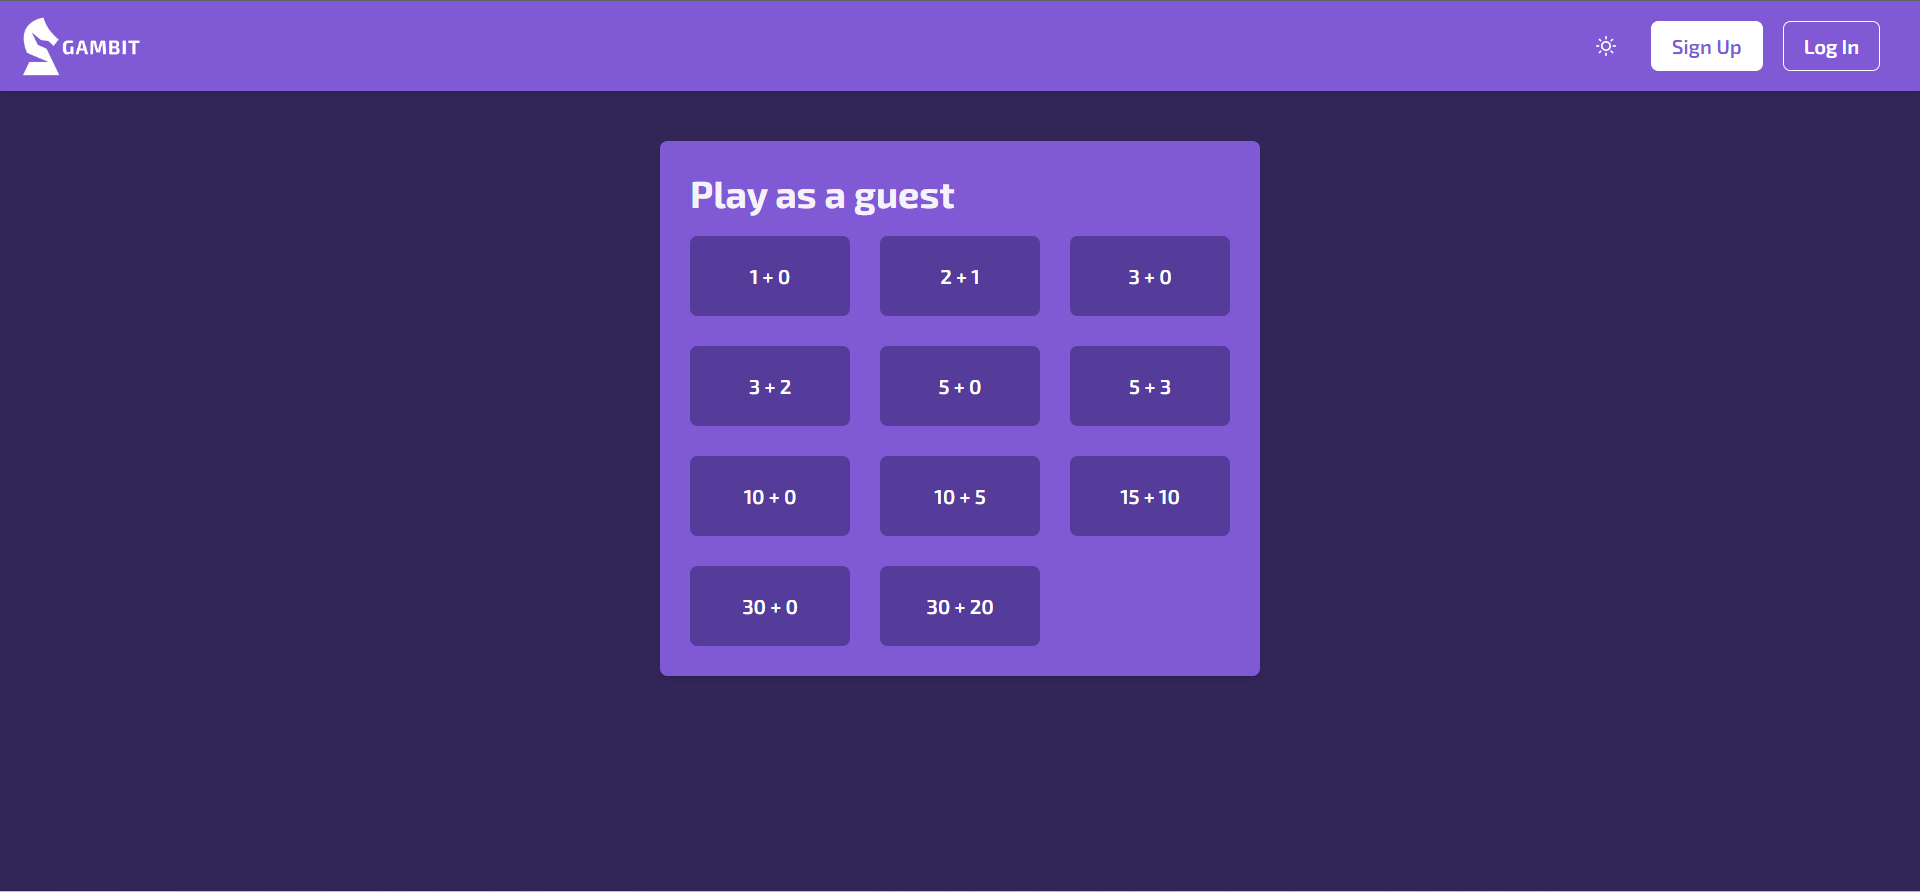
\includegraphics[width=\textwidth]{Home_not_logged_in.png}
  \caption{Home und Navbar Komponente eines nicht angemeldeten Benutzers im dunklen Farbschema}
  \label{fig:home-not-logged-in}
\end{figure}

  
    \begin{figure}[htbp]
    \centering
  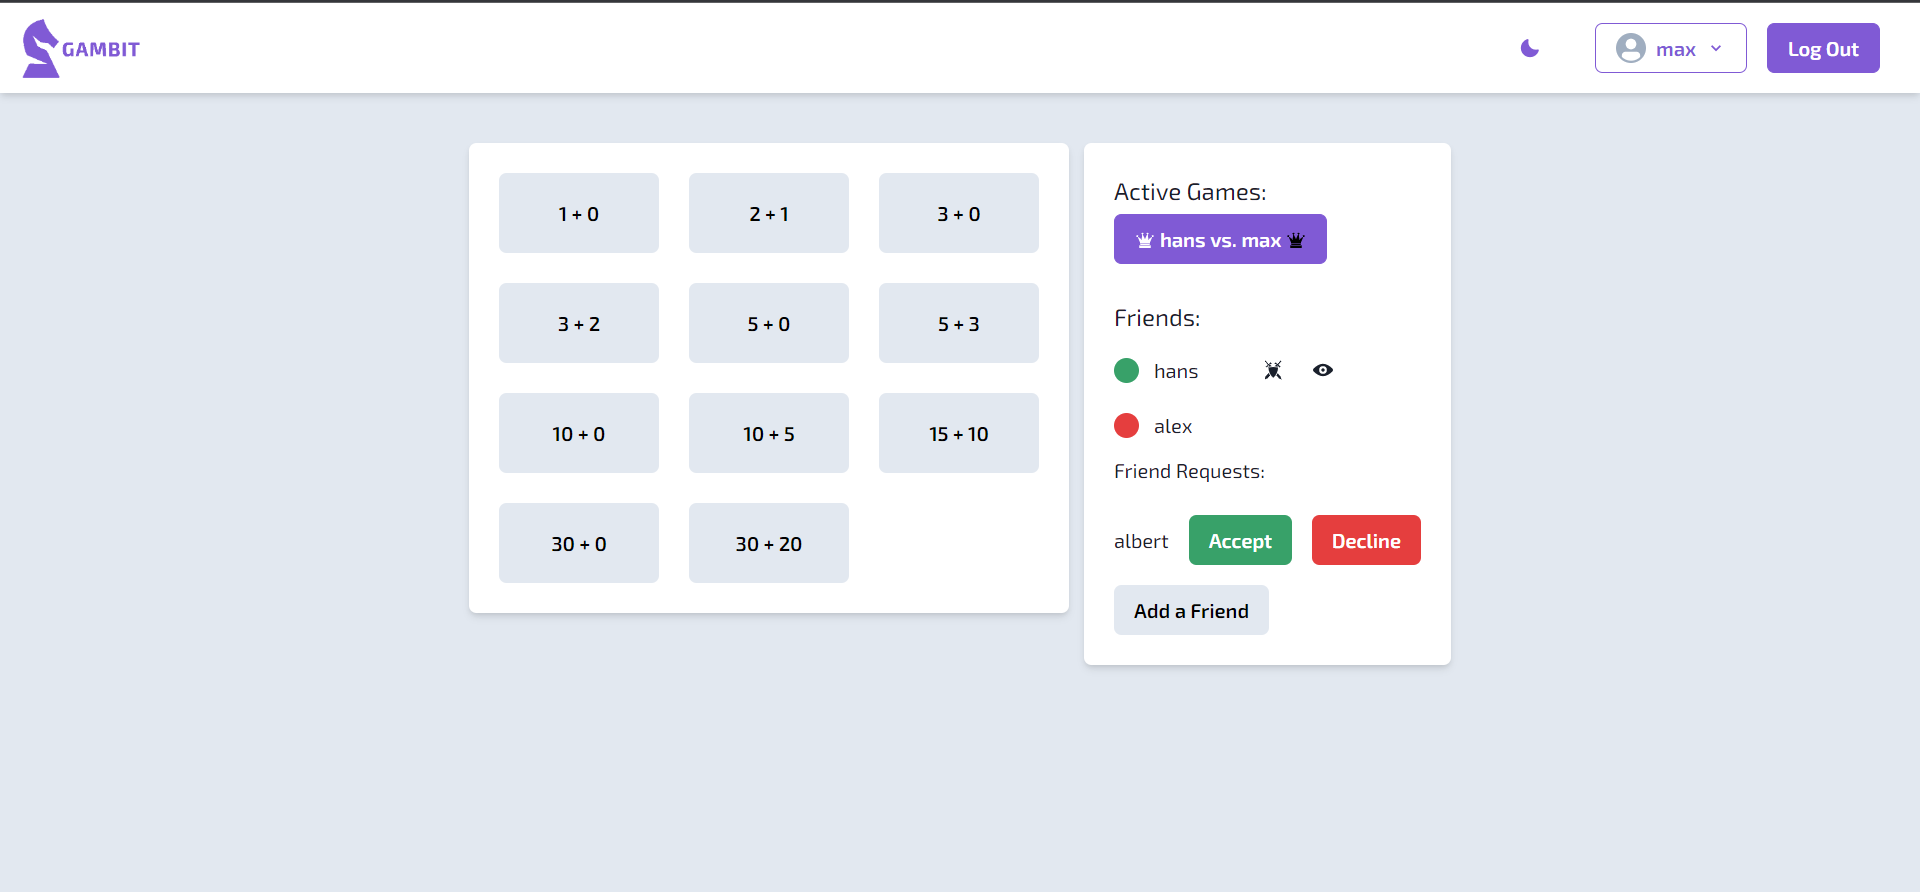
\includegraphics[width=\textwidth]{Home_logged_in.png}
  \caption{Home und Navbar Komponente eines angemeldeten Benutzers im hellen Farbschema}
  \label{fig:home-logged-in}
\end{figure}

      \begin{figure}[htbp]
      \centering
  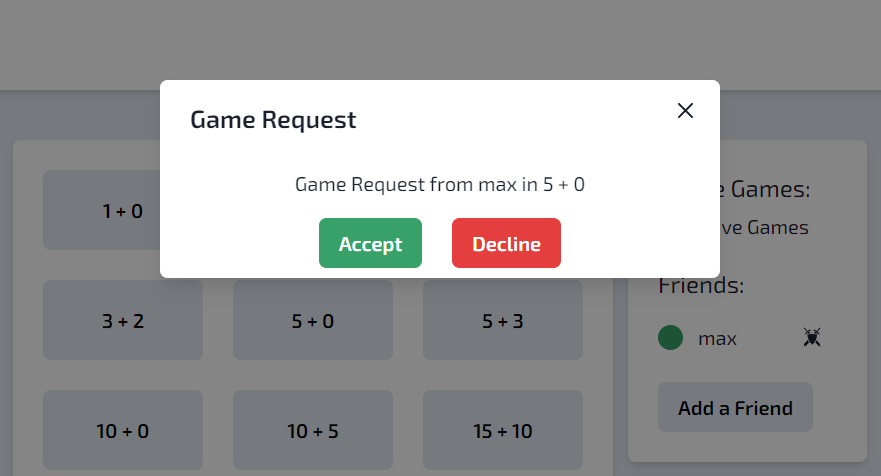
\includegraphics[width=0.7\textwidth]{game_request.png}
  \caption{Das Modal der Komponente GameRequest in hellem Farbschema}
  \label{fig:game-request}
\end{figure}

      \begin{figure}[htbp]
      \centering
  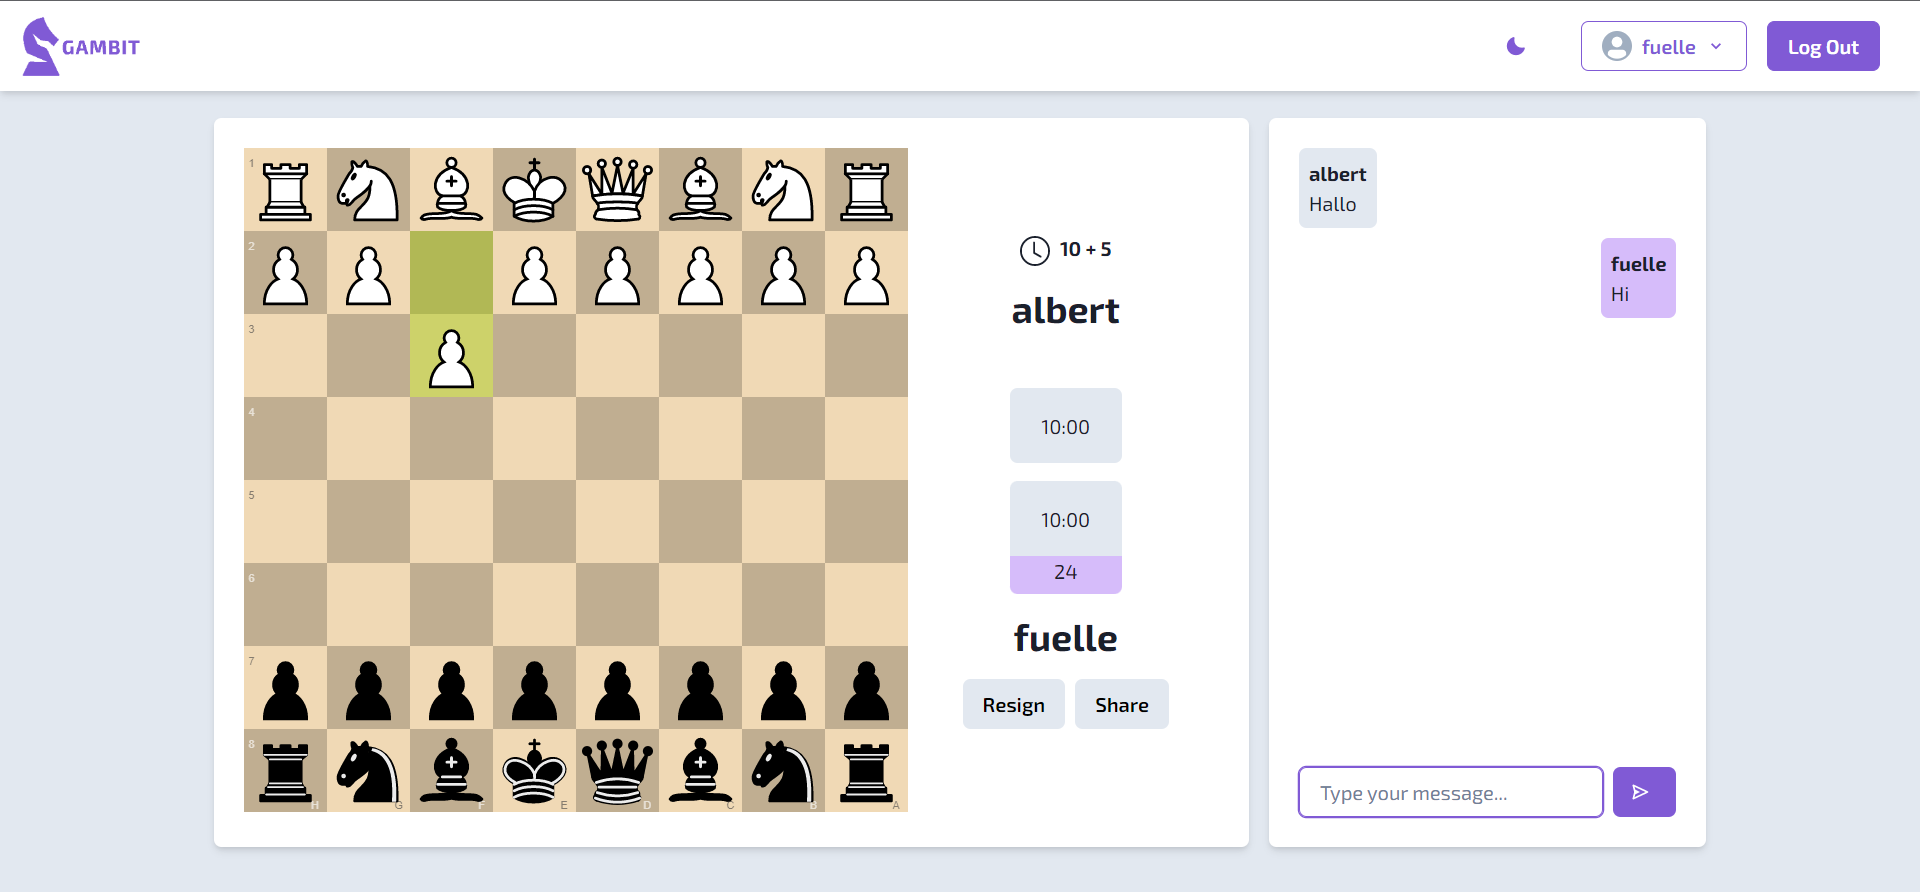
\includegraphics[width=\textwidth]{ChessGame.png}
  \caption{Beispiel einer ChessGame-Komponente} 
  \label{fig:chess-game}
\end{figure}
        

    
   
   \subsection{Authentifizierung}
   \label{sec:Autehtifizierung Frontend}
Die Authentifizierung findet in drei Komponenten statt: Dem \textit{UserContext} und den \textit{Login}- und \textit{SignUp}-Komponenten. Gewissermaßen hat \textit{SocketContext} auch etwas mit der Authentifizierung zu tun, da sobald sich der Anmeldezustand sich verändert eine neue socket Verbindung hergestellt wird. Was im Backend bei einer Authentifizierung stattfindet, wird in Abschnitt \ref{sec:Authentifizierung Backend} erläutert.

Der \textit{UserContext} beinhaltet den State \verb|user| und der \textit{SocketContext} beinhaltet den State \verb|socket|, welche beide mit \verb|null| initialisiert werden und den Komponenten zur Verfügung gestellt wird.
Nach dem rendern der Komponente wird im \textit{UserContext} eine GET HTTP Anfrage an den Server unter dem Pfad \verb|/auth/login| gesendet. Diese beinhaltet, falls vorhanden, den Cookie mit dem auf dem Server authentifiziert werden kann. Daraufhin sendet der Server die Antwort, ob der Benutzer nun angemeldet ist oder nicht und wenn ja, dann seinen Benutzernamen.
Dies wird in den \verb|user|-State gesetzt.

Wurde der \verb|user| gesetzt, wird im \textit{SocketContext} eine socket Verbindung hergestellt. Solange eine der beiden States der Kontexte \verb|null| ist, wird ein Lade-Bildschirm gezeigt, um fehlerhafte Darstellungen oder Funktionen zu vermeiden.

Die Authentifizierung der \textit{Login}- und \textit{SignUp}-Komponenten ist simpel gehalten. Mittels Formik und Yup (siehe Abschnitt \ref{sec:weiteres}) werden die Formulare überprüft und gegebenenfalls als POST HTTP Anfrage unter \verb|/auth/signup| oder \verb|/auth/login| an den Server gesendet. Falls es dabei auf dem Server einen Fehler gab, wird die Fehlermeldung angezeigt oder man erhält als Antwort die Benutzerdaten, welche in den \textit{UserContext} gespeichert werden. Auch hier wird nach dem Ändern des \verb|user| States in der \textit{UserContext}-Komponente eine neue socket Verbindung in \textit{SocketContext} hergestellt.
        
        \subsection{Das Schachspiel}
        \label{sec:Schachspiel}
        In diesem Kapitel werde ich näher darauf eingehen wie das Schachspiel im Frontend verwaltet und aktualisiert wird. Die Vorgehensweise im Backend und im Zusammenspiel finden Sie //REFERENZ
        
Das Schachspiel und die zugehörigen Schachuhren sind getrennt gehalten um die Modularität zu erhöhen. Die Schachuhren und das Spiel haben jeweils eigene Events und Listener auf die sie hören.
		\subsubsection{Das Starten eines Schachspiels}
		\label{sec:Frontend-Schach-Start}
Um eine Schachpartie zu starten können entweder die Buttons in der Mitte des Bildschirms der \textit{Home}-Komponente (siehe Abbildung \ref{fig:home-logged-in}) oder die Herausforderung/Annahme zu einer Partie eines Freundes verwendet werden.

Beim klicken auf eines der Zeitkonfigurations-Buttons in der \textit{Home}-Komponente wird das Event \verb|find_game| mit dem aktuellen Benutzerzustand der \textit{UserContext}-Komponente und der Auswahl der Zeitkonfiguration gesendet. Solange man auf einen zufälligen Gegner wartet erscheint ein Lade-Bildschirm, mit einem Button um den Suchvorgang eines Gegners abzubrechen (siehe Abbildung \ref{fig:searching-for-opponent}).

\begin{figure}[h]
\centering

\includegraphics[width=\textwidth]{searching-for-opponent.png}
\caption{Lade-Bildschirm beim Starten eines Spiels mit den Buttons der \textit{Home}-Komponente}
\label{fig:searching-for-opponent}
\end{figure}

Wurde ein Gegner für diese Zeitkonfiguration gefunden, wird in der \textit{Home}-Komponente das Event \verb|joined_game| mit der roomId unter der das Spiel stattfindet und gegebenenfalls einen Gast Benutzernamen empfangen und man wird zu dem Pfad \verb|/game/roomId| weitergeleitet, auf dem eine entsprechende \textit{ChessGame}-Komponente das Schachspiel initialisiert.

Wie man einen Freund zu einer Partie herausfordert und was passiert wenn der Freund die Anfrage akzeptiert oder ablehnt wird in Abschnitt \ref{sec:friend-komponente} erläutert, da dies eine Funktion ist, welche in der \textit{Friend}-Komponente stattfindet.

Wenn man selbst eine Anfrage erhält wird dies mittels der \textit{GameReqeust}-Komponente dargestellt (siehe Abbildung \ref{fig:game-request}). Diese besteht aus einer Liste aller gültigen Anfragen zu einer Partie und hat Listener auf die Events \verb|game_request| und \verb|cancel_game_request|. 

Das Event \verb|game_request| empfängt eine Anfrage zu einer Partie mit den Informationen um welche Zeitkonfiguration es sich handelt und wer einen herausfordert. Diese wird ganz einfach der Liste hinzugefügt. 

Das Event \verb|cancel_game_request| wird empfangen, sobald der Freund seine Anfrage zurück zieht. Es enthält den Benutzernamen des Spielers, der die Anfrage gesendet hat und diese Anfrage wird aus der Liste der Anfragen entfernt.

Gesendet werden kann das Event \verb|game_request_response| mit den Informationen um welche Anfrage es sich handelt und ob man die Anfrage akzeptiert oder ablehnt.
        \subsubsection{Das Spiel}
Das Schachspiel findet in der Komponente \textit{ChessGame} statt.
Nach dem rendern der Komponente wird das \verb|get_game_data| Event mit der roomId des Spiels und einer Callback Methode gesendet, die die Daten des Spiels beinhaltet, falls dieses existiert. Falls diese Partie nicht im Backend existiert, also keine Daten gesendet werden, wird der Benutzer darauf hingewiesen.

Die Daten die gesendet werden umfassen folgendes:
\begin{itemize}
\item Der Namen des weißen und des schwarzen Spielers.
\item Welcher Zeitmodus gespielt wird (z.B.: 5 + 3, 10 + 5, ...)
\item Die aktuelle Stellung der Partie
\item Die bisherigen Nachrichten im Chat.
\item Die aktuelle Phase des Spiels: Dabei gibt es die vier Möglichkeiten, dass die Startzeit von Schwarz oder Weiß läuft oder dass die reguläre Zeit von Schwarz oder Weiß läuft.
\item Die aktuellen Zeiten der Spieler.
\end{itemize}
Diese Informationen werden für den Fall benötigt, dass man die Seite neu lädt, über die \verb|ActiveGames|-Komponente auf die Seite gelangt, über einen Link der Partie beitritt oder ähnliches. Das Einholen dieser Daten gewährleistet, dass man auch in diesen Fällen noch ohne Veränderungen weiterspielen oder zugucken kann.

Aufgrund der gesendeten Namen der Spieler wird entschieden, ob man ein Zuschauer oder ein Spieler ist.  Dafür werden die Benutzernamen mit dem eigenen Benutzernamen im \textit{UserContext} verglichen. Doch was passiert wenn man eine Partie als unangemeldeter Benutzer spielt und deshalb keinen Benutzernamen im \textit{UserContext} hat?

Bei dem Event \verb|joined_game| (siehe Abschnitt \ref{sec:game-suche}) wird der Gast-Benutzername des Spielers mitgesendet und in \verb|location.state| gesetzt. Dadurch kann in der \textit{ChessGame}-Komponente darauf zugegriffen werden und es kann Überprüft werden, ob es sich um einen Spieler oder Zuschauer handelt.


Dem entsprechend wird auch bestimmt wie das Schachbrett, die Namen und die Schachuhren ausgerichtet sind. Ist man Zuschauer wird in chessground definiert, dass man keine Figuren bewegen kann und es gibt kein input Feld für den Chat, sodass man keine Nachrichten abschicken kann. Dies verhindert, dass ein Zuschauer Tipps geben könnte.

Zum Spielen der Partie werden folgende Listener definiert:
\begin{itemize}
\item \verb|opponent_move|: Dient zu Empfangen eines Zugs eines Spielers.
\item \verb|checkmate|: Ein Event welches bei Schachmatt mit dem Benutzernamen des Gewinners empfangen wird.
\item \verb|time_over|: Ist eine Benachrichtigung, dass die Zeit eines Spielers abgelaufen ist.
\item \verb|draw|: Kommuniziert ein Patt der Partie.
\item \verb|resigned|: Signalisiert, dass ein Spieler aufgegeben hat.
\item \verb|cancel_game|: Das Spiel wird aufgrund der abgalaufenen Start Zeit abgebrochen.
\end{itemize}
Die Events \verb|checkmate|, \verb|time_over|, \verb|draw|, \verb|resigned| und \verb|cancel_game| beschreiben alle das Ende des Schachspiels. In ihren Listenern wird definiert, dass man keine Figur des Schach Interfaces von chessground mehr bewegen darf und man wird über den Ausgang des Spiels in Form von einem Toast benachrichtigt. //BILD

Der Ablauf beim Empfangen eines neuen Zugs ist im Aktivitätsdiagramm in Abbildung \ref{fig:chess-opponent-move} dargestellt. Die Bauernumwandlung und das En Passant müssen separat behandelt werden, da chessground nur das Schach Interface zur Verfügung stellt und bei diesen beiden Zusatzregeln andere Figuren ersetzt oder entfernt werden, als bei regulären Zügen. Das aktualisieren möglicher Züge beinhaltet, dass chessground alle möglichen Züge von chess.js übertragen bekommt, welches zur Folge hat, dass bei einem Klick auf eine Figur korrekt angezeigt wird wohin diese Figur ziehen könnte und auch nur auf diese Felder kann eine Figur bewegt werden (siehe Abbildung \ref{fig:chess-game}).

Gesendet werden können die Events: \verb|new_move| zum senden eines Zugs, \verb|resign| zum Aufgaben der Partie und \verb|leave_room|, wenn der Spieler die \textit{ChessGame} Komponente verlässt.
Ein Aktivitätsdiagramm des Senden eines Zugs befindet sich in Abbildung \ref{fig:chess-move}. Genau wie bei dem Empfangen eines Zugs wird auch beim Senden zwischen Bauernumwandlung und En Passant unterschieden. Der einzige Unterschied ist, dass bei der Bauernumwandlung nach dem setzen des Zuges noch mittels der  \textit{PromotionModal}-Komponente ausgewählt werden muss, in welche Figur sich der Bauer umwandeln soll, bevor der Zug gesendet wird.

Das Event zum Aufgeben wird nach dem klicken des \glqq resign\grqq{ }Buttons gesendet.


      \begin{figure}[h]
      \centering
  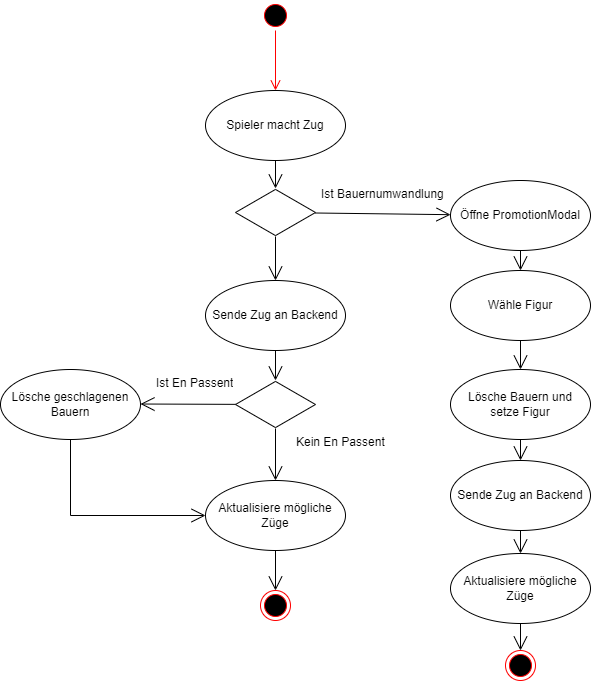
\includegraphics[width=0.8\textwidth]{Interaktion Schach Zug.png}
  \caption{Aktivitätsdiagramm eines Schach Zugs}
  \label{fig:chess-move}
\end{figure}

      \begin{figure}[h]
      \centering
  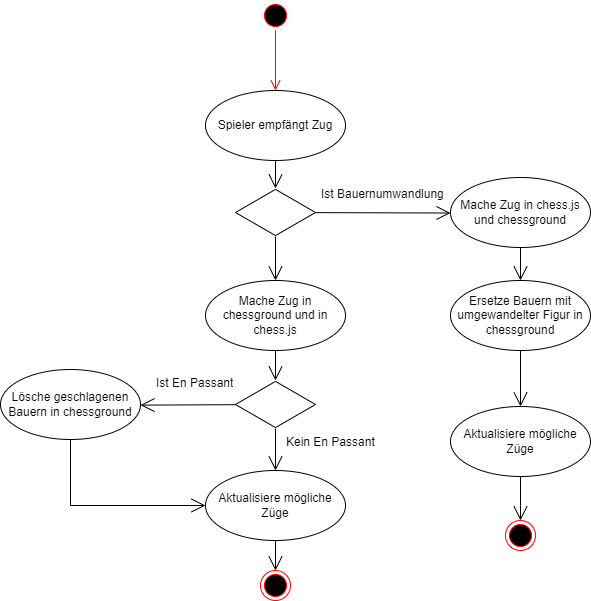
\includegraphics[width=0.8\textwidth]{Interaktion Schach Zug empfangen.png}
  \caption{Aktivitätsdiagramm eines empfangenen Schach Zugs}
  \label{fig:chess-opponent-move}
\end{figure}

        \subsubsection{Die Uhr}
Die \textit{ChessClock} Komponente bekommt von \textit{ChessGame} als Props die aktuelle Phase der Partie, die jeweiligen aktuellen Zeiten und die Ausrichtung, welche Zeit oben bzw. unten gezeigt werden soll. Neben der regulären Schach Zeit gibt es noch eine Startzeit, welche während des ersten Zugs jeden Spielers abläuft, um zu gewährleisten, dass das Spiel auch erst wirklich startet sobald beide Spieler bereit sind. Läuft die Startzeit ab wird das Spiel abgebrochen (siehe Abschnitt \ref{sec:schach-theorie}). Diese Startzeit ist die lila eingefärbte Zeit in Abbildung \ref{fig:chess-game}.

Die Komponente sendet keine Events, sondern hört nur auf die folgenden:
\begin{itemize}
\item \verb|updated_time|: Dieses Event wird vom Backend gesendet, sobald ein Zug gemacht wurde und enthält die aktuellen Zeiten der Spieler nach dem Zug und welcher Spieler jetzt am Zug ist. Dementsprechend werden die Zeiten aktualisiert und die Uhr des Spielers, welcher jetzt dran ist wird gestartet.
\item \verb|stop_starting_time_white|: Stoppt die Start Zeit des weißen Spielers und startet die Start Zeit des schwarzen Spielers.
\item \verb|stop_starting_time_black|: Stoppt die Start Zeit des schwarzen Spielers und lässt die reguläre Zeit des weißen Spielers beginnen.
\item \verb|stop_clocks|: Wird bei Beendung des Spiels empfangen und stoppt die aktive Uhr.
\end{itemize}

\subsubsection{Der Chat}
Die \textit{Chat}-Komponente bekommt als props alle bisher gesendeten Nachrichten, die Id unter der das Spiel stattfindet, die Information ob es sich um einen Zuschauer handelt und gegebenenfalls den Gastnamen, falls es sich um einen nicht angemeldeten Benutzer handelt. Handelt es sich um einen Zuschauer wird das Input-Feld der Komponente nicht angezeigt, um keine Nachrichten schreiben zu können. Die Komponente ist relativ simpel und sendet das Event \verb|send_message|, um eine Nachricht zu senden und empfängt eine Nachricht mit dem \verb|message| Event. Eine Nachricht beinhaltet immer den Namen des Versenders, die Nachricht als String und die roomId des Spiels. Je nachdem ob der Versendet der Nachricht mit dem eigenen Namen übereinstimmt wird die Nachricht unterschiedlich ausgerichtet und eingefärbt (siehe Abbildung \ref{fig:chess-game}).

\subsection{Verwaltung von Freunden}
\label{sec:Friends}
Die Verwaltung und Darstellung (siehe Abbildung \ref{fig:home-logged-in}) von Freunden und Freundschaftsanfragen obliegt der \textit{FriendList}-Komponente. Diese Beinhaltet die Unterkomponenten \textit{Friend}, \textit{FriendReqeust} und \textit{AddFriendModal}.

\subsubsection{\textit{FriendList}-Komponente}

\textit{FriendList} verwendet zwei States in Form von Arrays: \verb|friends| und \verb|friendRequests|. Je ein Element dieser Listen wird durch eine \textit{Friend}, beziehungsweise \textit{FriendRequest}, Komponente dargestellt und verwaltet. \textit{FriendList} hört dabei auf die folgenden Events: 
\begin{itemize}
\item \textbf{friends:} Ein Event welches nach der Anmeldung des Nutzers empfangen wird, um die Liste der Freunde zu bekommen.
\item \textbf{friend\_requests:} Genau das gleiche Event, nur zum setzen der Freundschaftsanfragen.
\item \textbf{friend\_request\_accepted:} Enthält Daten eines neuen Freundes, welcher deine Freundschaftsanfrage angenommen hat. Dieser wird der Freundesliste hinzugefügt.
\item \textbf{friend\_request:} Eingang einer neuen Freundschaftsanfrage. Wird der Liste der Freundschaftsanfragen hinzugefügt.
\item \textbf{connected:} Dieses Event wird empfangen, falls ein Freund von dir offline, beziehungsweise online geht. Der betreffende Freundes-Eintrag in der Freundesliste wird aktualisiert.
\end{itemize}

Des weiteren werden die zwei Events \verb|get_friends| und \verb|get_friend_requests| jedes Mal gesendet, falls auf den Pfad \verb|/| navigiert wird auf der sich die \textit{Home}-Komponente befindet. Diese beiden Events empfangen mittels Callback-Funktion alle Daten über die Freunde und Freundschaftsanfragen. Dies ist nötig, damit, falls beispielsweise nach einer Schachpartie wieder auf die \textit{Home}-Komponente navigiert wird, die Daten der Freunde aktualisiert werden.

\subsubsection{\textit{Friend}-Komponente}
\label{sec:friend-komponente}
Diese Komponente stellt einen Freund dar. Es kriegt als props alle wichtigen Daten des Freundes gestellt. Sie hat zwei Grundlegende Funktionen: Das Zuschauen einer Partie eines Freundes und das Herausfordern zu einer Partie. Beim Herausfordern eines Freundes sind genau die gleichen Schachuhren möglich, wie bei der Suche eines zufälligen Gegners und das Zuschauen ist Aufgebaut wie bei der \textit{ActiveGames}-Komponente. (siehe Abbildung \ref{fig:Freunde-zuschauen-herausfordern})

Diese beiden Funktionen sind nur verfügbar, falls der Freund gerade online ist, welches über einen grünen Punkt ersichtlich ist.

Die Komponente hat zwei Eventlistener: \verb|game_request_accepted| und \verb|game_request_denied|, welche einen Toast darstellen und den Spieler gegebenenfalls zu dem Spiel navigieren. 

Senden tut die Komponente zwei Events: \verb|send_game_request| und \verb|cancel_game_request|. Wurde eine Herausforderung zu einer Partie versendet erscheint ein Lade-Bildschirm, bis der Spieler die Anfrage angenommen, beziehungsweise abgelehnt hat. Entscheidet sich der Spieler davor doch nicht mehr gegen den Freund zu spielen, kann er auf den \glqq Cancel\grqq{ }Button klicken und die Spielanfrage wird zurückgenommen.

\begin{figure}[h]
\centering
  \begin{subfigure}[c]{0.35\textwidth}
  \centering
  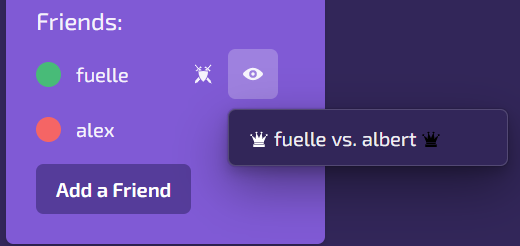
\includegraphics[width=\linewidth]{activeGames-friends.png}
  \caption{Aktive Partien eines Freundes}
  \label{fig:activeGames-friends}
  \end{subfigure}
  \hfill
  \begin{subfigure}[c]{0.3\textwidth}
  \centering
    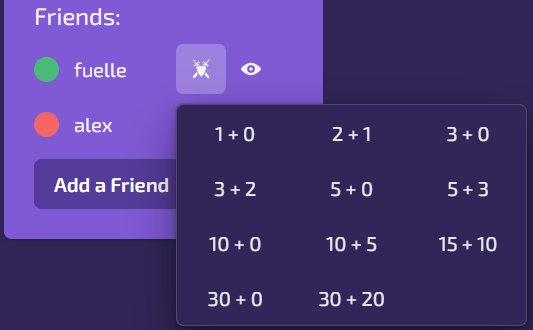
\includegraphics[width=\linewidth]{Spiel-herausfordern.png}
  \caption{Das Herausfordern eines Freundes}
  \label{fig:spiel-herausfordern}
  \end{subfigure}
  \hfill
 \begin{subfigure}[c]{0.3\textwidth}
  \centering
    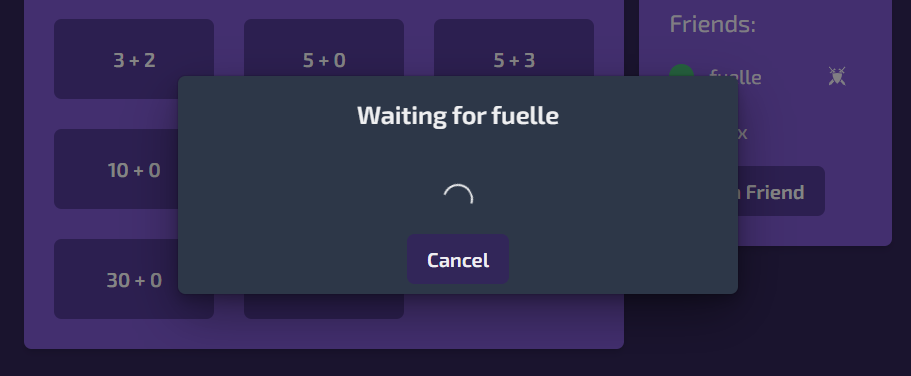
\includegraphics[width=\linewidth]{waiting-for-friend.png}
  \caption{Warte auf Freund Modal}
  \label{fig:waiting-for-friend}
  \end{subfigure}
  \caption{Das Herausfordern und Zuschauen bei Freunden}
  \label{fig:Freunde-zuschauen-herausfordern}
 
\end{figure}


\subsubsection{\textit{FriendRequest}-Komponente}
Die \textit{FriendRequest}-Komponente stellt eine Freundschaftsanfrage dar und erhält ebenfalls seine Daten von der \textit{FriendList}-Komponente, wozu auch die Funktionen \verb|setFriends| und \verb|setFriendRequest| zählen, um die Listen der \textit{FriendList}-Komponente zu ändern.
Es hört auf keine Events, sendet allerdings zwei Events: \verb|accept_friend_request| und \verb|decline_friend_request|. Die Behandlung dieser Events im Backend wird in Abschnitt \ref{sec:accept-friend-request} erläutert. War das Akzeptieren, beziehungsweise das Ablehnen der Anfrage erfolgreich wird die Freundschaftsanfrage aus der Liste gelöscht und zusätzlich wird gegebenenfalls der neue Freund der Freundesliste hinzugefügt.

\subsubsection{\textit{AddFriendModal}-Komponente}
Diese Komponente besteht aus einem Button und einem Modal, falls man den Button anklickt. In diesem Modal kann man einen Benutzernamen angeben, an den die Freundschaftsanfrage verschickt werden soll. Das Versenden einer Freundschaftsanfrage wird mittels des \verb|send_friend_request| Events erledigt und behandelt. Es beinhaltet eine Callback-Funktion, welche entgegennimmt, ob die Versendung erfolgreich war und wenn nicht, dann eine Fehlermeldung, warum es nicht möglich war die Freundschaftsanfrage zu versenden (siehe Abbildung \ref{fig:AddFriendModal}). Wie das Backend eine neue Freundschaftsanfrage behandelt wird in Abschnitt \ref{sec:hinzufügen-von-Freunden} erläutert.

\begin{figure}[h]
\centering
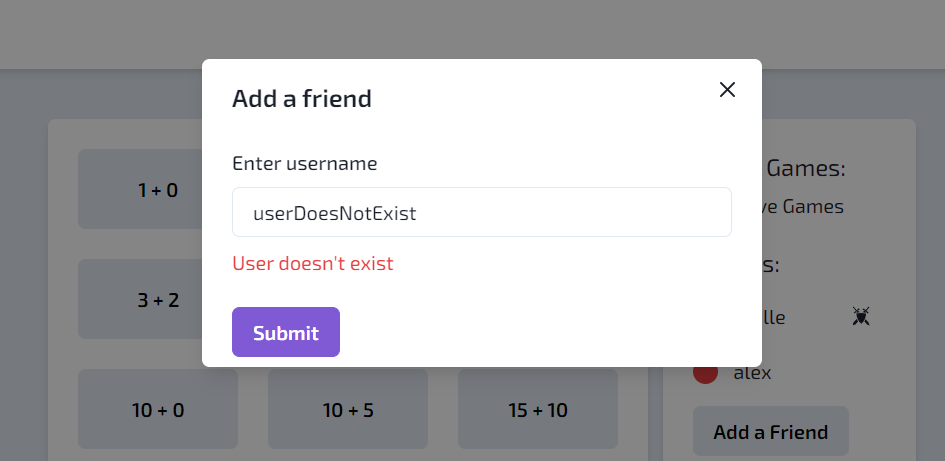
\includegraphics[width=0.7\textwidth]{AddFriendModal.png}
\caption{Das Modal der \textit{AddFriendModal}-Komponente mit Fehlermeldung}
\label{fig:AddFriendModal}
\end{figure}

\subsection{Anzeigen und navigieren zu aktiven Partien}
Falls man eine aktive Schachpartie spielt und aus Versehen den Browser schließt, auf die Startseite navigiert oder ähnliches gäbe es keine Möglichkeit auf das Spiel zurück zu kehren, es sei denn man hat den Link oder die Id des Spiels gespeichert. Um es möglich zu machen auf aktive Spiele schnell wieder zurück zu kehren gibt es die Unterkomponente \textit{ActiveGames} in der \textit{Home}-Komponente (siehe Abbildung \ref{fig:home-logged-in}). Diese Komponente macht es möglich zu verfolgen welche offenen Spiele man gegen wen in welcher Farbe hat und man kann leicht wieder zu diesen Spielen navigieren, indem man auf den Button klickt.
Es besitzt den Listener auf das Event \verb|active_games|, welches nach einer erfolgreichen socket Authentifizierung (siehe Abschnitt \ref{sec:socketauth}) mit einer Liste aller aktiven Spiele gesendet wird. Des weiteren sendet es das Event \verb|get_active_games|, welches mit einer Callback Funktion ebenfalls so eine Liste empfängt. Dieses Event wird, wie bei dem Event \verb|get_friends| von der \textit{FriendList}-Komponente, gesendet, falls wieder auf die \textit{Home}-Komponente navigiert wird, um die Liste der aktiven Spiele zu aktualisieren.
Ist die Liste leer, wird nur \glqq No acitve Games\grqq{ } angezeigt. Ansonsten wird jedes aktive Spiel der Liste mit einem Button dargestellt, auf deren klick man zu dem Spiel navigiert wird.

        \section{Backend-Architektur}
Das Backend basiert auf Node.js mit dem Express Framework. Des weiteren werden als Schnittstellen mit dem Frontend eine Web-API für HTTP Anfragen und ein Socket.io Server bereitgestellt. Das Backend kommuniziert mit zwei Datenbanken: einer PostgreSQL Datenbank für die Benutzerverwaltung und eine Redis Datenbank für häufig aktualisierte und angefragte Daten.

Die Ordnerstruktur des Backends (Abbildung \ref{fig:backend_dirtree}) ist auf dieser Weise aufgebaut:

\begin{itemize}
\item \textbf{auth:} Dieser Ordner beschäftigt sich sowohl mit der Schnittstelle der Web-API Kommunikation mit dem Frontend, als auch deren Behandlung und dem Austausch mit der PostgreSQL Datenbank. Diese Schnittstellen dienen bloß der Anmeldung und Registrierung eines Benutzers.
\item \textbf{chess:} Stellt ein chess.js Schachspiel zur Verfügung und die serverseitige Schachuhr.
\item \textbf{redis:} Dient als Schnittstelle und Verwalter von Operationen auf der redis Datenbank.
\item \textbf{sockets:} Stellt Middleware für die Verbindungsherstellung und Listener für die Kommunikation zwischen Frontend und Backend bereit.
\item \textbf{index.js:} Initialisiert den Server mit seinen Schnittstellen.
\end{itemize}

\begin{figure}[h]
\centering

\begin{minipage}{0.5\textwidth}
\dirtree{%
.1 server/.
.2 src/.
.3 auth/ .
.4 authController.js.
.4 database.js.
.4 rateLimiter.js.
.4 validateForm.js.
.3 chess/.
.4 Chess.mjs.
.4 ServerChessClock.js.
.3 redis/.
.4 redis.js.
.4 redisController.js.
.3 routers/.
.4 authRouter.js.
.3 sockets/.
.4 socketChessController.js.
.4 socketController.js.
.4 socketMiddleware.js.
.2 .env.
.2 index.js.
.2 package.json.
}
\end{minipage}
\caption{Ordnerstruktur des Backends}
\label{fig:backend_dirtree}

\end{figure}


\subsection{Authentifizierung}
\label{sec:Authentifizierung Backend}
Die Authentifizierung eines Benutzers läuft über HTTP Anfragen an die Web-API und einer PostgreSQL Datenbank.
Nachdem die erste Authentifizierung stattgefunden hat wird die Socket.io Verbindung des Clients hergestellt, in der der Benutzer nochmals Authentifiziert wird.
Es gibt drei verschiedene Möglichkeiten wie ein Benutzer authentifiziert werden kann: Durch das Anmelden, durch das Registrieren oder durch das Lesen des Cookies beim Aufruf der Seite vom Client.

Die Authentifizierung im Frontend abläuft wird in Abschnitt \ref{sec:Autehtifizierung Frontend} erläutert.

\subsubsection{Authentifizierung mit der Web-API und PostgreSQL}
Das Anmelden und Registrieren mittels Formular läuft über eine POST Anfrage des Clients an den Pfad \verb|/auth/login|, beziehungsweise \verb|/auth/signup|, die die angegebenen Formulardaten beinhaltet. Bei der Verarbeitung der Anfrage werden mittels des Express Routing verschiedene Middlewares verwendet.

Eine Middleware stellt sicher, dass die Anzahl der Anfragen über eine IP-Adresse in einer bestimmten Zeit begrenzt wird. Dies verhindert sogenannte Denial-of-Service (kurz: DoS) Attacken\footnote{Quelle: \url{https://www.bsi.bund.de/DE/Themen/Verbraucherinnen-und-Verbraucher/Cyber-Sicherheitslage/Methoden-der-Cyber-Kriminalitaet/DoS-Denial-of-Service/dos-denial-of-service_node.html} am 27. April 2023}, bei denen probiert wird den Server mit so vielen Anfragen zu belasten, dass dieser außer Betrieb gesetzt wird.

Anschließend überprüft eine Middleware, ob die angegebenen Daten mit dem Schema übereinstimmen. 

Treten bei diesen beiden Middlewares keine Fehler auf wird beim Anmelden überprüft, ob dieser Benutzer in der Datenbank existiert und es wird mittels bcrypt überprüft ob die Passwörter übereinstimmen. Ist dies der Fall, wird ein JWT-Token mit den Benutzerinformationen erstellt und als Cookie in den Browser des Clients gesetzt. Des weiteren wird dem Benutzer natürlich geantwortet, dass die Anmeldung erfolgreich war.

Beim Registrieren wird überprüft, ob bereits ein Nutzer mit dem Benutzernamen oder E-Mail existiert und anschließend wird ein neuer Tupel in der PostgreSQL Datenbank erstellt, der Cookie mit dem JWT-Token gesetzt und dem Benutzer geantwortet.

Bei dem ersten Aufruf der Seite vom Client wird eine GET Anfrage an \verb|/auth/login| gestellt. Bei dieser wird ebenfalls die Middleware gegen DoS-Attacken verwendet und anschließend wird überprüft, ob er einen gültigen JWT-Token im Cookie hat und ihm wird dem entsprechend geantwortet. Das setzen des Tokens im Cookie hat den Vorteil, dass beim neuen Aufruf der Seite, solange der Cookie noch gültig ist, der Benutzer automatisch angemeldet wird, ohne seine Anmeldedaten nochmals einzugeben.

Anschließend stellt der Client eine Socket.io Verbindung her.

\subsubsection{Authentifizierung und anschließende Middleware mit Socket.io}
\label{sec:socketauth}
Bei der Verbindungsherstellung des Clients mit dem Socket.io Server durchläuft die socket verschiedene Middlewares.

Die erste Middleware Authentifiziert die Socket des Benutzer. Sie liest aus dem Cookie, der auch in der socket mitgesendet wird, den JWT-Token, falls dieser existiert. Die Daten die in dem Token kodiert sind werden dann in der Socket als Attribute gesetzt, sodass anschließend immer mittels \verb|socket.user| darauf zugegriffen werden kann.

Wenn der Benutzer keinen gültigen JWT-Token hat, werden trotzdem alle Middlewares ohne Fehler durchlaufen. Dies liegt daran, dass bei einem fehlgeschlagenen Middleware-Prozess die Socket.io-Verbindung abgelehnt werden würde. Es soll allerdings auch das Spielen einer Schachpartie als Gast möglich sein.

Als zweite Middleware wird der Benutzer mit Daten versorgt, er tritt dem Raum seiner userid bei und wird als online vermerkt. Dabei wird in Redis \verb|user:username| mit seinen Informationen und \verb|connected true| gesetzt. Anschließend werden alle Freunde des Benutzers aus der Redis Datenbank geholt und an alle ein Event gesendet, das signalisiert, dass der Benutzer online ist. Des weiteren werden auch Informationen bezüglich aktiver Spiele und Freundschaftsanfragen aus Redis abgerufen und mittels entsprechenden Events werden die Informationen über Freunde, aktive Partien und Freundschaftsanfragen an den Benutzer gesendet.

Als letzte Middleware werden alle nötigen Listener sowohl für das Schachspiel, als auch für sonstige Funktionen initialisiert.

\subsection{Hinzufügen von Freunden}
\label{sec:hinzufügen-von-Freunden}
In den Aktivitätsdiagrammen in Abbildung \ref{fig:Freunde-backend} ist der Ablauf des Versenden und Akzeptieren einer Freundschaftsanfrage abgebildet.
Die verschiedenen Datentypen der Speicherung in Redis befindet sich in Abschnitt \ref{sec:redis-data}.

\subsubsection{Versenden einer Freundschaftsanfrage}
Beim Versenden einer Freundschaftsanfrage wird vom Frontend das Event \verb|send_friend_request| mit dem angegebenen Benutzernamen versendet. Um zu überprüfen, ob eine Freundschaft der beiden erlaubt ist, wird kontrolliert, ob es der eigene Benutzername ist, ob der Nutzer existiert und ob die beiden Benutzer schon befreundet sind. Ist eines davon nicht der Fall, wird mit einer entsprechenden Fehlernachricht dem Sender mittels einer Callback Funktion geantwortet. 
Ist die Freundschaft erlaubt wird zusätzlich noch überprüft ob es noch eine offene Freundschaftsanfrage zwischen den beiden gibt und falls dies der Fall wird, wird der Benutzer ebenfalls darauf hingewiesen.
Ansonsten wird die Freundschaftsanfrage in Redis gespeichert und ein Event mit der Freundschaftsanfrage wird an den betreffenden Spieler gesendet und der Sender wird darüber informiert, dass die Freundschaftsanfrage versendet wurde.

\subsubsection{Akzeptieren und Ablehnen einer Freundschaftsanfrage}
\label{sec:accept-friend-request}
Beim Akzeptieren einer Freundschaftsanfrage wird wie bei dem Versenden nochmals überprüft, ob diese Freundschaft erlaubt ist. Anschließend wird die Freundschaftsanfrage gelöscht, die beiden Benutzer werden in die entsprechende Freundesliste gesetzt, die restlichen Daten der beiden Spieler werden eingeholt und an beide Benutzer werden alle Informationen, wie ob sie online sind oder ob sie aktive Spiele haben, an beide gesendet. Dies stellt sicher, dass sie im Frontend direkt richtig angezeigt werden können.

Beim Ablehnen einer Freundschaftsanfrage wird einfach nur die Freundschaftsanfrage aus Redis gelöscht.

      \begin{figure}[h!]
      \centering
      \begin{subfigure}[b]{0.35\textwidth}
      \centering
  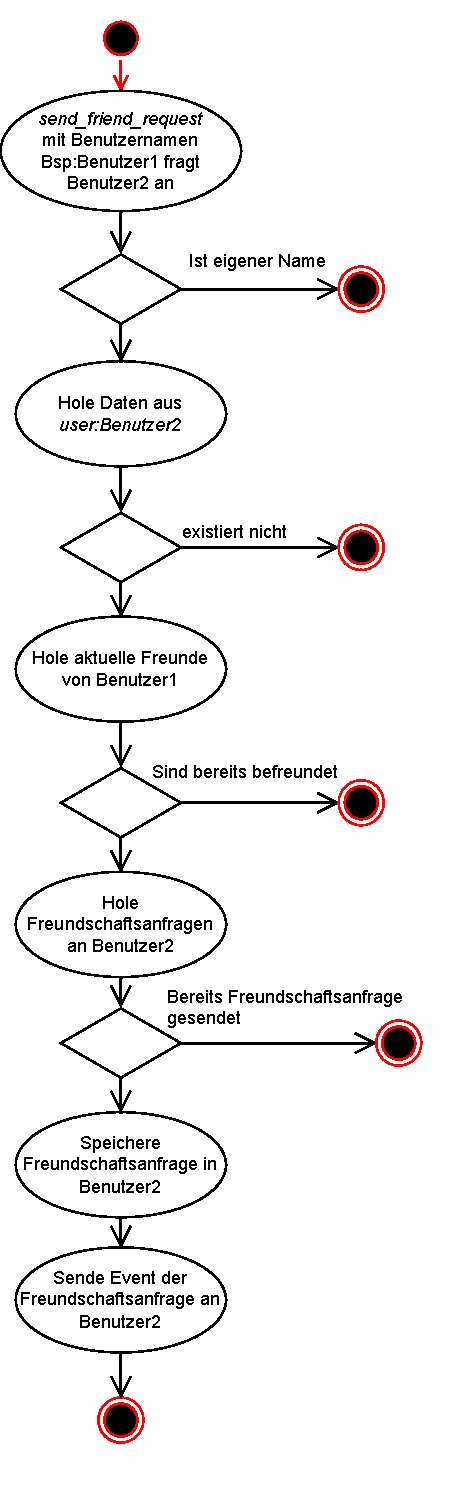
\includegraphics[width=\linewidth]{Freunde-adden.pdf}
  \caption{Senden einer Freundschaftsanfrage}
  \label{fig:friend_request}
  \end{subfigure}
  \hspace{10mm}
  \begin{subfigure}[b]{0.3\textwidth}
  \centering
    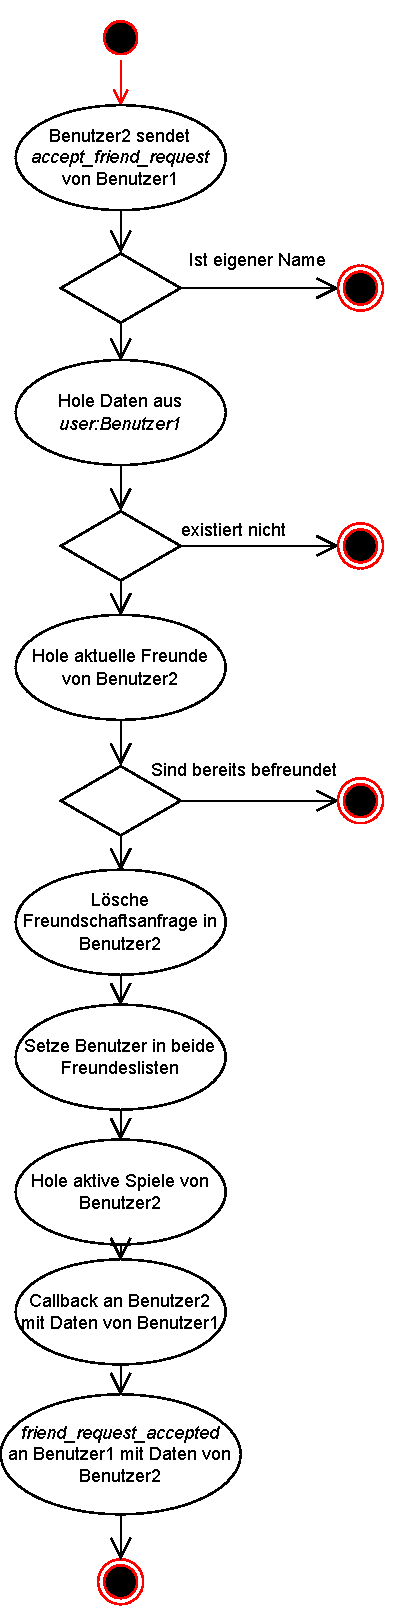
\includegraphics[width=\linewidth]{Freund akzeptieren.pdf}
  \caption{Akzeptieren einer Freundschaftsanfrage}
  \label{fig:friend_request}
  \end{subfigure}
  \caption{Aktivitätsdiagramme des Versenden und Akzeptieren von Freundschaftsanfragen}
  \label{fig:Freunde-backend}
 
\end{figure}

\subsection{Das Schachspiel}
In diesem Abschnitt erkläre ich, was genau beim initialisieren, bei neuen Zügen und neuen Nachrichten im Chat eines Schachspiels passiert. Eine Erklärung wie das Frontend und Backend miteinander kommuniziert um ein Gegner zu finden befindet sich in Abschnitt \ref{sec:game-suche}.

\subsubsection{Finden eines Gegners}
Es gibt 3 verschiedene Arten ein Schachspiel zu starten: Ein angemeldeter Benutzer sucht einen zufälligen Gegner, ein angemeldeter Benutzer spielt ein Spiel gegen einen Freund und ein unangemeldeter Benutzer spielt gegen einen zufälligen Gegner.

Das Suchen eines Spiels mit zufälligem Gegner wird mittels des Events \verb|find_game| mit den Benutzerdaten und der gewählten Zeitkonfiguration vom Frontend gesendet. Ein Sequenzdiagramm des starten eines Spiels mit zufälligem Gegner befindet sich in Abbildung \ref{fig:sequence_chess_start}. Dies beinhaltet folgende Schritte:
     
\begin{figure}[h!]
  \centering
  
 
\begin{adjustbox}{width=\textwidth}
  \begin{sequencediagram}[scale=0.2]
    \newinst{clientA}{Client A}
    \newinst[2]{clientB}{Client B}
    \newthread{server}{Server}
    \tikzstyle {inststyle}+=[rounded corners=3mm]
    \newinst[3]{redis}{Redis DB}
    
    \begin{messcall}{clientA}{find\_game}{server}
    \begin{call}{server}{getPlayerInQueue}{redis}{player}
    \end{call}
    
    \begin{sdblock}{Kein Spieler in der Warteschlange}{}
    	\begin{messcall}{server}{addPlayerInQueue}{redis}{}
    	\end{messcall}
    	\end{sdblock}
    	
    	\begin{messcall}{clientB}{find\_game}{server}{}
    	\end{messcall}
    	
    \begin{call}{server}{getPlayerInQueue}{redis}{player}
    \end{call}
    	
    	\begin{sdblock}{Spieler in Warteschlange}{}
    \begin{callself}{server}{Erstelle Spiel}{roomId}
    \end{callself}
    \postlevel
    	\begin{messcall}{server}{Speichere Spiel}{redis}
    	\end{messcall}
    	\prelevel
    	\begin{messcall}{server}{joined\_game, roomId}{clientA}{}
    	\prelevel\prelevel
    	\mess{clientA}{navigiere zu /game/roomId}{clientA}
    	\postlevel\postlevel
    	\begin{call}{clientA}{get\_game\_data, roomId}{server}{gameData}
    	\begin{call}{server}{Hole Daten des Spiels}{redis}{gameData}
    	\end{call}
    	\end{call}
    	\end{messcall}
    	\prelevel
    	\begin{messcall}{server}{}{clientB}{}
    	\begin{call}{clientB}{}{server}{}
    	\begin{call}{server}{}{redis}{}
    	\end{call}
    	\end{call}
    	\end{messcall}
    	\end{sdblock}
    \end{messcall}
    
    
    
  \end{sequencediagram}
  \end{adjustbox}
  
  \caption{Sequenzdiagramm des Schachspielstartprozesses mit unbekanntem Gegner}
  \label{fig:sequence_chess_start}
\end{figure}


\begin{itemize}
\item Das Event \verb|find_game| mit der Zeitkonfiguration und Benutzerdaten wird gesendet (siehe Abschnitt \ref{sec:Frontend-Schach-Start}).
\item Falls der Benutzer nicht angemeldet ist, wird ihm  ein zufälliger username für dieses Schachspiel zugewiesen, der mit \glqq guest-\grqq{ }startet. Seine userid wird als seine socket id festgelegt.
\item Daraufhin wird im Server ein Spieler aus der entsprechenden Warteschlange aus Redis genommen (siehe Abschnitt \ref{sec:Warteschlange}).
\item Falls dabei kein Spieler entnommen werden konnte, wird der Benutzer selbst in die Liste geschrieben und wartet bis er von einem anderen Benutzer aus der Liste genommen wird.
\item Falls ein Spieler aus der Liste entnommen werden konnte, wird das Spiel mit einer \textit{roomId} als Identifikator initialisiert und in Redis gespeichert.
\item An die beiden Spieler wird das Event \verb|joined_game| mit der roomId und gegebenenfalls dem Gast-Benutzernamen gesendet, woraufhin sie zu dem Pfad \verb|/game/roomId| navigieren, auf der sich die \textit{ChessGame}-Komponente befindet.
\item Die \textit{ChessGame}-Komponente sendet das \verb|get_game_data| Event. Daraufhin wird der aktuelle Zustands der Partie aus Redis geholt und an das Frontend zurück gesendet. Ein Ablauf was im Frontend bei einer Schachpartie passiert befindet sich im Abschnitt \ref{sec:Schachspiel}.
\end{itemize}

Falls es sich um eine Partie handelt, die aus einer Herausforderung eines Freundes resultiert, wird natürlich in keine Warteschlange nach einem Gegner gesucht, anstatt dessen wird mit den Events \verb|send_game_request|, \verb|game_request| und \verb|game_request_response| (siehe Abschnitt \ref{sec:friend-komponente}, \ref{sec:Frontend-Schach-Start}) die Anfrage versendet und beantwortet. Anschließend wird das Spiel initialisiert und an die beiden Spieler das Event \verb|game_request_accepted| mit der roomId gesendet.

\subsubsection{Initialisieren eines Spiels nach gefundenem Gegner}
Zunächst wird per Zufall entschieden welcher Spieler weiß und welcher Spieler schwarz spielt. Anschließend wird ein neues Schachspiel der Klasse chess.js (siehe Abschnitt \ref{sec:chess.js}) erstellt und in ihr festgehalten welcher Spieler weiß, beziehungsweise schwarz, spielt und das Datum an dem dieses Spiel stattfindet. Des weiteren wird eine zufällige roomId generiert, unter der das Schachspiel stattfindet.

Der weitere Ablauf der Initialisierung wird im Sequenzdiagramm in Abbildung \ref{fig:sequenz-initialize-Game} dargestellt. 

\begin{figure}[h]
\centering
\begin{tikzpicture}
\begin{umlseqdiag}

\umlobject[no ddots]{socketChessController}
\umlobject[no ddots]{redisController}
\umldatabase[no ddots]{Redis DB}

\begin{umlcall}[op=initializeGame]{socketChessController}{redisController}
\begin{umlcall}[op=game:roomId]{redisController}{Redis DB}
\end{umlcall}
\begin{umlfragment}[type=Angemeldet]
\begin{umlcall}[op=activeGames:username]{redisController}{Redis DB}
\end{umlcall}
\begin{umlcall}[op=activeGames:username]{redisController}{Redis DB}
\end{umlcall}
\end{umlfragment}
\end{umlcall}

\umlcreatecall[no ddots]{socketChessController}{ServerChessClock}

\begin{umlcall}[op=starStartingTimer('white')]{socketChessController}{ServerChessClock}
\end{umlcall}

\end{umlseqdiag}
\end{tikzpicture}
\caption{Sequenzdiagramm des Initialisieren eines Schachspiels}
\label{fig:sequenz-initialize-Game}
\end{figure}

Dem \textit{redisController} wird aufgetragen das Spiel in Redis zu initialisieren. Dafür bekommt er die Informationen darüber welcher Spieler welche Farbe spielt, unter welcher roomId das Spiel stattfindet und die bisherige PGN-Notation wird aus dem chess.js Objekt. Diese Informationen speichert er in Redis unter \verb|game:roomId| (siehe Abschnitt \ref{sec:game:roomId}) und falls die spieler angemeldet sind wird die roomId auch der Liste \verb|activeGames:username| bei beiden Spielern hinzugefügt.

Anschließend wird ein Objekt der Klasse ServerChessClock erstellt und die Startzeit des weißen Spielers gestartet. Das ServerChessClock Objekt wird in einem Array in der socketChessController Datei gespeichert, sodass mit der roomId darauf zugegriffen werden kann. Das Objekt ServerChessClock kommuniziert mittels Events mit socketChessListener und es werden folgende Eventlistener in socketChessListener definiert:
\begin{itemize}
\item \verb|cancel_game|: Das Spiel wird aufgrund einer abgelaufenen Startzeit abgebrochen.
\item \verb|time_over_white|:  Die Zeit des weißen Spielers ist abgelaufen.
\item \verb|time_over_black|:  Die Zeit des schwarzen Spielers ist abgelaufen.
\end{itemize}

Dies sind alles Ausgänge von Schachpartien, die an alle sockets im Raum weitergeleitet werden. Daraufhin wird das Schachspiel beendet (siehe Abschnitt \ref{sec:Schach-Ende}).

\subsubsection{ServerChessClock}
Die Klasse ServerChessClock definiert einzelne Schachuhr Objekte, welche die Startzeiten und die regulären Schachuhren verwalten.

socketChessController und ServerChessClock kommunizieren mittels Funktionen und Events miteinander, wobei Events genutzt werden um laufende Uhren anzuhalten und zu kommunizieren, dass eine Startzeit oder eine reguläre Schachuhr abgelaufen ist, während die Funktionsaufrufe von ServerChessClock dazu dienen eine bestimmte Zeit zu starten.

\subsubsection{Neuer Zug einer Schachpartie}
Ein Aktivitätsdiagramm zur Behandlung eines neuen Zuges im Backend ist in Abbildung \ref{fig:Zug-Backend} zu finden. 


Sobald ein neuer Zug eines Spielers mit dem Event \verb|new_move| ankommt wird die ServerChessClock aus dem Array und das aktuelle PGN aus der Redis Datenbank mittels der roomId geholt. Es wird ein neues chess.js Objekt kreiert, welches das aktuelle PGN importiert und anschließend den neuen Zug macht. Daraufhin wird der Zug in die roomId gebroadcastet. Das bedeutet, es wird an alle sockets im Raum gesendet, außer von dem Sender, da dieser ja bereits den Zug gemacht hat.

Nachdem der Zug gesendet wurde, wird überprüft ob es sich um ein Schachmatt oder ein Patt handelt, falls ja werden die Uhren der ServerChessClock angehalten, das Frontend wird über den Ausgang informiert und das Spiel wird beendet (siehe Abschnitt \ref{sec:Schach-Ende}). 

Falls dies nicht der Fall ist wird die Zeit des jetzigen Spielers gestoppt und falls es eine reguläre Zeit ist, wird das Inkrement auf die Zeit gerechnet, die Zeit des anderen Spielers fängt an zu laufen und die aktualisierten Zeiten werden an das Frontend gesendet.

Handelt es sich um die ersten zwei Züge, in denen die Startzeit und nicht die reguläre Zeit des Spielers läuft werden diese gesondert betrachtet und entweder die Startzeit von Schwarz beginnt zu laufen oder die reguläre Zeit von Weiß fängt an zu laufen. Dies wird auch mit entsprechenden Events dem Frontend mitgeteilt.

Als letztes wird noch die PGN-Notation mit dem neuen Zug in Redis gespeichert.


\begin{figure}[h!]
\centering
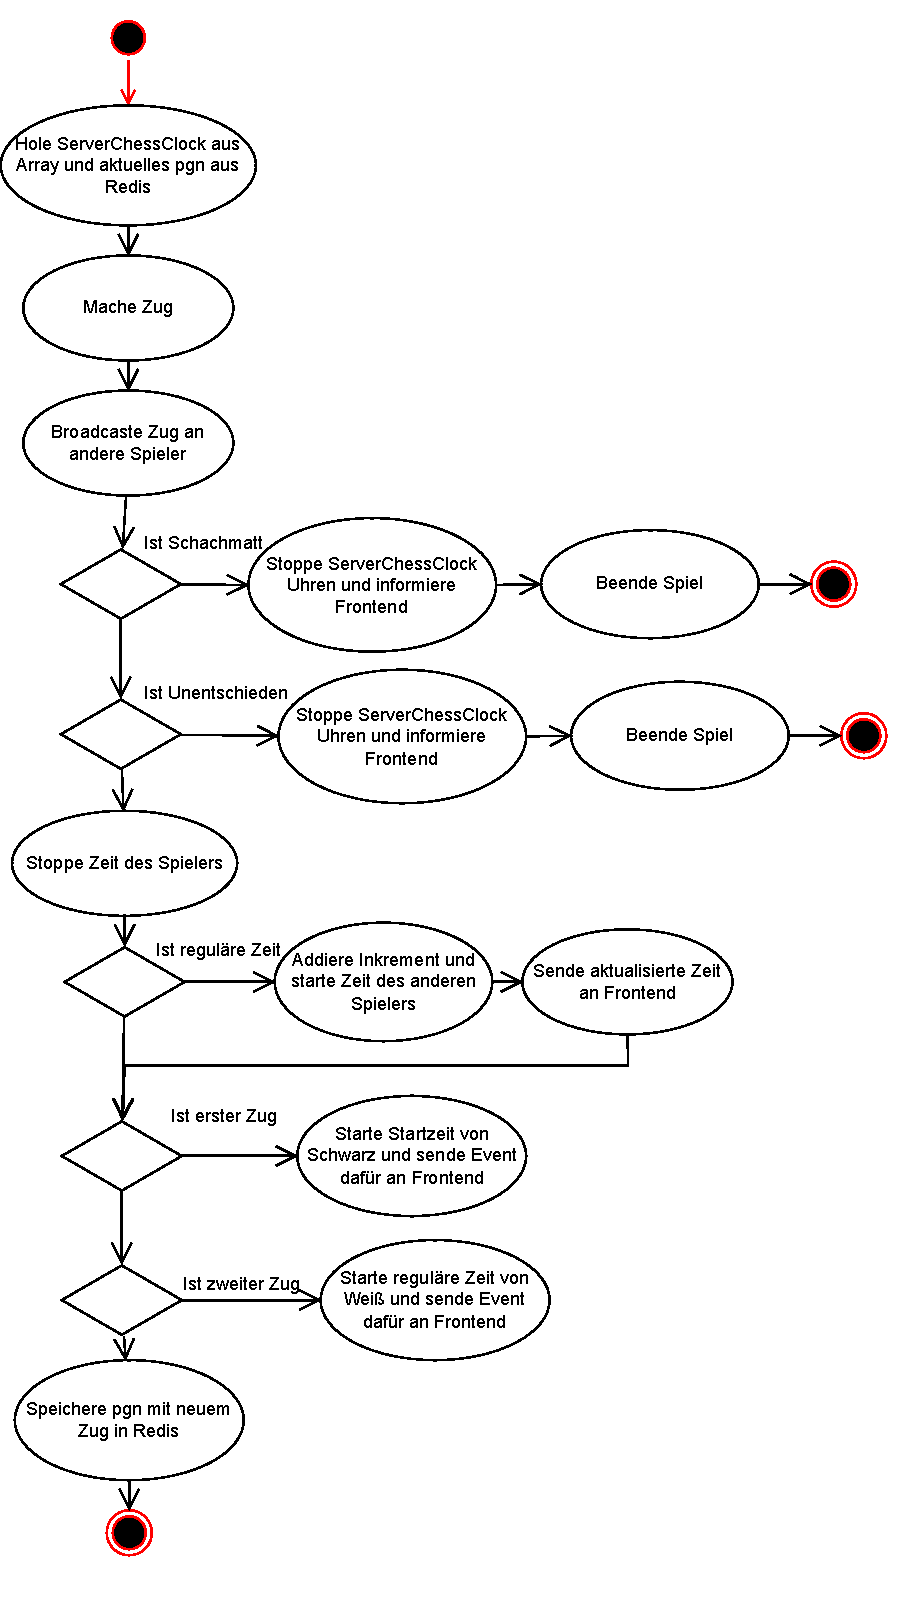
\includegraphics[width=0.8\textwidth]{Neuer Zug Backend.pdf}
\caption{Aktivitätsdiagramm zur Behandlung eines neuen Zuges im Backend}
\label{fig:Zug-Backend}
\end{figure}

\subsubsection{Ende einer Schachpartie}
\label{sec:Schach-Ende}
Das Ende einer Schachpartie kann durch folgende Situationen stattfinden:
Schachmatt, Patt, Startzeit ist abgelaufen, eine reguläre Zeit ist abgelaufen oder ein Spieler hat aufgegeben.

Auf Schachmatt und Patt wird bei neuen Zügen geachtet und an das Frontend gesendet. Wenn das Ende der Partie auf die Schachuhren zurückzuführen ist, wird ein Event von ServerChessClock in socketChessController empfangen und an die Sockets im Raum weitergeleitet. 

Bei einer Aufgabe empfängt das Backend das event \verb|resign| mit der Farbe welche aufgibt und der roomId und leitet dies entsprechend weiter.

Bei jedem dieser Ausgägnge einer Partie geschieht noch folgendes:

Das ServerChessClock Objekt wird aus dem Array in socketChessController gelöscht.

Die Benutzernamen werden aus dem Redis Eintrag \verb|game:roomId| geholt und falls es sich um angemeldete Benutzer handelt wird das entsprechende \verb|activeGames:username| Element aus der Liste gelöscht. Anschließend wird der Eintrag \verb|game:roomId| gelöscht.

Somit wird kein Speicher mehr von alten Spielen belegt.
		\section{Datenbankstruktur}
\subsection{PostgreSQL Datenbank}
Die PostgreSQL Datenbank wird ausschließlich für die Anmeldung und Registrierung genutzt. Sie enthält eine Tabelle mit folgendem Schema:
\begin{itemize}
\item \textbf{id:} Eine Fortlaufende id, die als Primärschlüssel dient.
\item \textbf{email:} Die E-Mail, die bei der Registrierung angegeben wurde.
\item \textbf{username:} Der Benutzername des Benutzers.
\item \textbf{userid:} Jeder Spieler erhält beim Registrieren seine eigene userid. Diese dient der Kommunikation mit dem Benutzer. Bei einer Verbindung mit Socket.io erhält die socket immer eine andere Id, also wie sendet man ein Event an einen bestimmten Spieler? Diese userid löst das Problem, indem man nach dem anmelden immer dieser id als Raum beitritt. Somit kann immer an diese Id gesendet werden und man stellt sicher, dass der Client das Event empfängt.
\item \textbf{password:} Das mit bcrypt verschlüsselte Passwort des Benutzers.
\end{itemize}
Jedes dieser Attribute, außer das Passwort, hat die Einschränkung, dass es einzigartig sein muss. Die E-Mail wird bisher nicht genutzt, kann aber in Zukunft zum Bestätigen der Registrierung oder Einrichtung eines Newsletters genutzt werden.

\subsection{Redis}
\label{sec:redis-data}
\subsubsection{user:username}
Unter dem Key \verb|user:username| (wobei hier \verb|username| mit dem entsprechenden Benutzernamen ausgetauscht wird) befindet sich ein Redis Hash. Ein Redis Hash besitzt Key-Value Paare, auf welche man zugreifen kann.

In unserem Fall werden folgende Values zu den Keys dort gespeichert:
\begin{itemize}
\item \textbf{userid:} Auch hier wird die userid gespeichert, da Redis vor allem für socket.io Funktionen verwendet wird und daher eine kurze Abfragezeit benötigt.
\item \textbf{connected:} Ist \glqq true\grqq{ } oder \glqq false\grqq , je nachdem ob der Benutzer gerade online ist oder nicht.
\end{itemize}

\subsubsection{game:roomId}
\label{sec:game:roomId}
Der Redis Hash \verb|game:roomId| verwaltet die Daten einer Schachpartie. Dazu gehören:
\begin{itemize}
\item \textbf{whitePlayer, blackPlayer:} Benutzernamen des weißen und schwarzen Spielers.
\item \textbf{time:} Der Zeitmodus welcher gespielt wird (z.B.: 15 + 10, 5 + 3, ...)
\item \textbf{pgn:} Die Historie aller bisherigen Züge im PGN Format.
\item \textbf{chat:} Alle bisher geschriebenen Nachrichten im Chat.
\end{itemize}

\subsubsection{activeGames:username}
\label{activeGames:username}
\verb|activeGames:username| beinhaltet eine Liste der aktiven Spiele dieses Benutzers. In der Liste stehen alle roomIds der aktiven Spiele.

\subsubsection{friends:username}
Der Key \verb|friends:username| verweist auf eine Liste von Freunden. Diese Freunde bestehen aus einem String, der sich zusammensetzt aus username:userid. Dies verhindert, dass wenn man ein Event an einen Freund senden will, man einen extra Zugriff auf user:username machen muss um die userid zu bekommen.

\subsubsection{friend\_requests:username}
Dies ist eine Liste die genauso aufgebaut ist wie die \verb|friends:username| Liste, außer, dass sie Freundschaftsanfragen verwaltet.

\subsubsection{Warteschlangen}
\label{sec:Warteschlange}
Die letzten Elemente sind die Warteschlangen für Spiele. Diese bestehen aus \verb|waitingPlayers:timeMode| und \verb|waitingGuests:timeMode|, je nachdem, ob es sich um einen angemeldeten Benutzer handelt oder nicht. \verb|timeMode| repräsentiert hier alle möglichen Schachuhren, also beispielsweise \glqq 10 + 5\grqq , \glqq 15 + 10\grqq , ...

Diese Warteschlagen sind Listen, welche aus \verb|username:userid| Einträgen bestehen, um die Anzahl an Abfragen zu verringern. 

Durch die Redis Operationen \verb|RPOP| und \verb|LPUSH| lassen sich atomar Einträge hinzufügen oder herausnehmen, welches die Konsistenz der Liste gewährleistet.